% DYSLEXIA SWITCH
\newif\ifdys
		
				% ENABLE or DISABLE font change
				% use XeLaTeX if true
				\dystrue
				\dysfalse


\ifdys

\documentclass[a4paper, 14pt]{extarticle}
\usepackage{amsmath,amsfonts,amsthm,amssymb,mathtools}

\tracinglostchars=3 % Report an error if a font does not have a symbol.
\usepackage{fontspec}
\usepackage{unicode-math}
\defaultfontfeatures{ Ligatures=TeX,
                      Scale=MatchUppercase }

\setmainfont{OpenDyslexic}[Scale=1.0]
\setmathfont{Fira Math} % Or maybe try KPMath-Sans?
\setmathfont{OpenDyslexic Italic}[range=it/{Latin,latin}]
\setmathfont{OpenDyslexic}[range=up/{Latin,latin,num}]

\else

\documentclass[a4paper, 12pt]{extarticle}

\usepackage[utf8x]{inputenc}
%fonts
\usepackage{amsmath,amsfonts,amsthm,amssymb,mathtools}
% comment below to default to computer modern
\usepackage{libertinus,libertinust1math}

\fi


\usepackage[french]{babel}
\usepackage[
a4paper,
margin=2cm,
nomarginpar,% We don't want any margin paragraphs
]{geometry}
\usepackage{icomma}

\usepackage{fancyhdr}
\usepackage{array}
\usepackage{hyperref}

\usepackage{multicol, enumerate}
\newcolumntype{P}[1]{>{\centering\arraybackslash}p{#1}}


\usepackage{stackengine}
\newcommand\xrowht[2][0]{\addstackgap[.5\dimexpr#2\relax]{\vphantom{#1}}}

% theorems

\theoremstyle{plain}
\newtheorem{theorem}{Th\'eor\`eme}
\newtheorem*{sol}{Solution}
\theoremstyle{definition}
\newtheorem{ex}{Exercice}
\newtheorem*{rpl}{Rappel}
\newtheorem{enigme}{Énigme}

% corps
\usepackage{calrsfs}
\newcommand{\C}{\mathcal{C}}
\newcommand{\R}{\mathbb{R}}
\newcommand{\Rnn}{\mathbb{R}^{2n}}
\newcommand{\Z}{\mathbb{Z}}
\newcommand{\N}{\mathbb{N}}
\newcommand{\Q}{\mathbb{Q}}

% variance
\newcommand{\Var}[1]{\text{Var}(#1)}

% domain
\newcommand{\D}{\mathcal{D}}


% date
\usepackage{advdate}
\AdvanceDate[0]


% plots
\usepackage{pgfplots}

% table line break
\usepackage{makecell}
%tablestuff
\def\arraystretch{2}
\setlength\tabcolsep{15pt}

%subfigures
\usepackage{subcaption}

\definecolor{myg}{RGB}{56, 140, 70}
\definecolor{myb}{RGB}{45, 111, 177}
\definecolor{myr}{RGB}{199, 68, 64}

% fake sections with no title to move around the merged pdf
\newcommand{\fakesection}[1]{%
  \par\refstepcounter{section}% Increase section counter
  \sectionmark{#1}% Add section mark (header)
  \addcontentsline{toc}{section}{\protect\numberline{\thesection}#1}% Add section to ToC
  % Add more content here, if needed.
}


% SOLUTION SWITCH
\newif\ifsolutions
				\solutionstrue
				%\solutionsfalse

\ifsolutions
	\newcommand{\exe}[2]{
		\begin{ex} #1  \end{ex}
		\begin{sol} #2 \end{sol}
	}
\else
	\newcommand{\exe}[2]{
		\begin{ex} #1  \end{ex}
	}
	
\fi


% tableaux var, signe
\usepackage{tkz-tab}


%pinfty minfty
\newcommand{\pinfty}{{+}\infty}
\newcommand{\minfty}{{-}\infty}

\begin{document}


\AdvanceDate[0]

\begin{document}
\pagestyle{fancy}
\fancyhead[L]{Seconde}
\fancyhead[C]{\textbf{Représenter des points dans le plan en Python}}
\fancyhead[R]{\today}

Le but de ce document est d'automatiser l'exercice \ref{exe:milieu-segment} de la feuille « Plan cartésien ».
Automatiser permet d'accélérer la vitesse de calcul en évitant les erreurs (en ignorant les erreurs probables du programmeur débutant).

\setcounter{Exercise}{11}
\exe{}{
	Représenter les points $A(1;1)$ et $B(3;-1)$ dans un repère orthonormé.
	Représenter le point
		\[ \lambda A + (1-\lambda)B, \]
	pour certaines valeurs de $\lambda$ (lu « lambda ») entre 0 et 1.
}{exe:milieu-segment}{}


\subsection*{Stocker un nombre}

Il faut utiliser le point à la place de la virgule pour séparer la partie décimale de la partie entière des nombres. C'est la notation utilisée notamment en Angleterre, aux États-Unis, en Inde, et en Chine\footnote{Voir la carte \href{https://en.wikipedia.org/wiki/Decimal_separator\#Conventions_worldwide}{https://en.wikipedia.org/wiki/Decimal\_separator\#Conventions\_worldwide}.}.
	\[ \dfrac12 = 0.5 \] 
Lorsqu'on écrit $x=0.5$, la valeur à droite du signe « = » est stocké dans la variable à gauche.

\warning Le signe « = » a un sens différent qu'en mathématiques. Il sert uniquement à stocker la valeur de droite dans la variable de gauche.

\subsection*{Définir et stocker une liste de nombres}

Une liste de nombres est créée avec des crochets. Les éléments sont séparés par des virgules.

Le signe « = » stocke la liste à droite dans la variable à gauche.

\texttt{list = [0, 1, 0.1, 0.5, 0.6]}

\subsection*{Parcourir une liste}

Pour parcourir une liste, on utilise la boucle \emph{for}.

Pour chaque élément de la liste, l'élément est stocké dans la variable, et tout le bloc est executé.

L'indentation est importante en Python car elle définit quelles lignes appartiennent ou non au bloc.

\subsection*{Multiplication est addition}

\texttt{x = $\lambda$*1 + (1-$\lambda$)*3}

\texttt{y = $\lambda$*1 + (1-$\lambda$)*(-1)}

\subsection*{Représentation dans un repère}

\texttt{import matplotlib.pyplot as plt}

\texttt{plt.scatter(x,y)}

\texttt{plt.show()}

\subsection*{Programme final}

\vspace{10cm}

\subsection*{Améliorations possibles}

Ajouter un quadrillage avec 
\texttt{plt.grid()}.

Remplacer la liste par \texttt{liste = [i/100 for i in range(101)]}.

Mettre le point en couleur pour connaître la valeur de $\lambda$.

%%%%%%%%%%%

\newpage
\fancyhead[C]{\textbf{Solutions}}


\begin{multicols}{2}
	\python{segment}
	\columnbreak
	\centering
	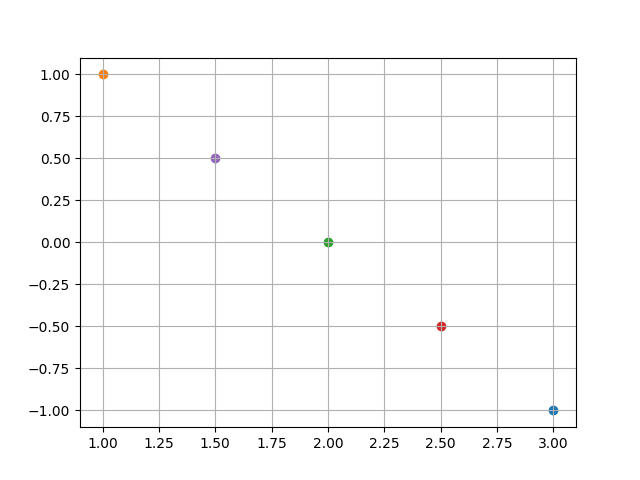
\includegraphics[scale=.7]{segment.png}
\end{multicols}

\begin{multicols}{2}
	\python{segment-ameliore}
	\columnbreak
	\centering
	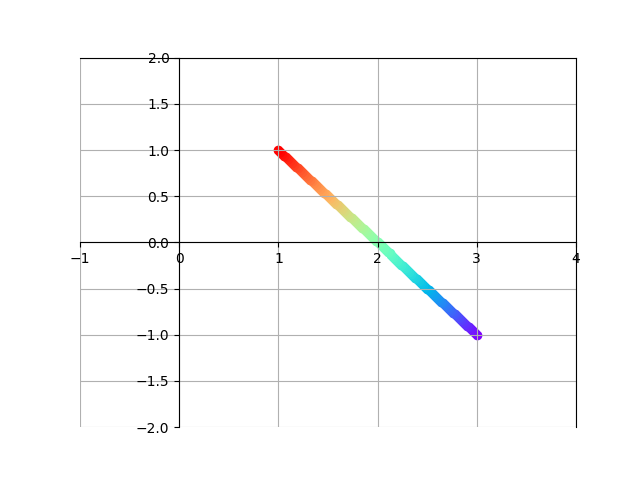
\includegraphics[scale=.6]{segment-ameliore.png}
\end{multicols}

\end{document}
